\documentclass{article}

\usepackage{epsfig}
\usepackage{graphicx}
\usepackage{xspace}
\usepackage{url}

\newcommand{\kw}[1]{\emph{#1}\xspace}

\newcommand{\appl}[1]{\textsl{#1}\xspace}

\newcommand{\swig}{\appl{Swig}}

\newcommand{\glade}{\appl{Glade}}

\newcommand{\pygtk}{\appl{PyGTK}}
\newcommand{\python}{\appl{Python}}

\newcommand{\mvco}{\kw{MVC--O}}
\newcommand{\mvc}{\kw{MVC} pattern\xspace}
\newcommand{\obs}{\kw{Observer} pattern\xspace}
\newcommand{\gui}{\kw{GUI}}
\newcommand{\pygtkmvc}{\kw{gtkmvc}}
\newcommand{\gtkmvc}{\kw{gtkmvc}}


\newcommand{\file}[1]{\texttt{#1}\xspace}

\newcommand{\codename}[1]{\texttt{\bfseries \small{#1}}\xspace}

\newcommand{\codesize}{\small}

\newcommand{\OP}{\kw{OP}}
\newcommand{\OPS}{\kw{OPs}}
\newcommand{\OPvar}{\codename{\_\_properties\_\_}}
\newcommand{\OPdvar}{\codename{\_\_derived\_properties\_\_}}
\newcommand{\OBSvar}{\codename{\_\_observables\_\_}}


\begin{document}

\title{Model-View-Controller and Observer patterns for \pygtk \\
Version 1.99.0}

\author{ Roberto Cavada \thanks{FBK-irst, Trento, Italy,
 cavada@fbk.eu} }

\maketitle

\tableofcontents

\newpage

% ----------------------------------------------------------------------
\section{Introduction}

This document contains information about the functionalities and the
architecture of a Model-View-Controller and Observer Infrastructure
(\mvco from here on) for \pygtk version 2. The aim is to supply the
essential information in order to make developers able to effectively
use, modify and extend the infrastructure, in order to easily create
new applications based on it.

\bigskip

Section \ref{MOT} tries to motivate the usage of \pygtkmvc, by
discussing the context which the framework is thought to operate, and
its main goals.

Section \ref{ARCH} briefly gives an overview of the general
architecture for a \gui application based on Python and the GTK
toolkit, showing all major parts, and how these depend on each other.
In this general picture, the proposed \mvco framework is also
collocated, to provide an initial idea of how an hypothetical
application based on it should be organized.

Section \ref{MVCO} describes the basement of a \gui application, the
\mvco Infrastructure. 

Finally, Sections \ref{DI} and \ref{SAP} supply some further details
about implementation, via many examples. The examples aim to make more
concrete the ideas described in all previous sections.


% ----------------------------------------------------------------------

\newpage
% ----------------------------------------------------------------------
\section{Motivations}
\label{MOT}

One major effort of Software Engineering has been to provide a way of
optimally separating the logical parts that constitute a software.
This issue becomes a question of outstanding importance in
middle/large interactive software, where an agent like an human user
interacts with the software, likely through a Graphic User Interface
(\gui).
To separate the logic (data) of an application from the representation
of those data, several Architectural Patterns
\footnote{\url{http://en.wikipedia.org/wiki/%
    Architectural_pattern_\%28computer_science_\%29}} 
have been studied; one is the Model--View--Controller (MVC) pattern
that splits the application into three separate parts, the \kw{Model},
the \kw{View} and the \kw{Controller}. The level of mutual knowledge
among these three entities is kept as minimal as possible, and this
results in:

\begin{itemize}
\item Reduced wrong dependencies.
\item Software architecture forced to be better designed.
\item Minimized propagation of changes/modifications.
\item Higher costs of startup, but potential lower costs of
  maintenance.
\end{itemize}


To improve re-usability and robustness of software, the \obs is used
as well. This pattern identifies two entities: the
\emph{Observable data} and the \emph{Observer} over those data.\\
The implementation of the \obs is intended to make the Observer take
some action when the Observable data change. This triggering mechanism
is a further abstraction layer that helps to
design and implement robust software.\\
A possible use of the \obs is in combination with the \mvc, where the
model communicates indirectly with the presentation side through the
observer pattern.

\smallskip

\pygtkmvc is a framework that implements both the MVC and Observer
patterns to be used to produce middle/large applications in Python and
\pygtk. \\
The main goal is to provide a minimal (but not trivial)
implementation, where practical aspects are taken into serious
consideration, and complexity is kept behind the scene. This makes the
users able to mainly focus their attention on the application they
need to produce, instead of dealing with the underlying framework.

\bigskip Pointless to say that goals are clear and likely easy to
share by anyone. It is quite a different thing to prove that those
goals are reached by the proposed framework. Frankly, this is up to
the reader to decide.


% ----------------------------------------------------------------------

\newpage
% ----------------------------------------------------------------------
\section{\label{ARCH} Architectural Overview}

Figure \ref{HLA_f} shows the high level software architecture for an
application based on \pygtk and the supplied {mvco} Infrastructure. It
shows the functional architecture as well.

\begin{figure}[htbp]
\begin{center}
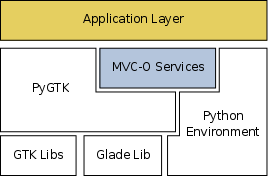
\includegraphics[width=8cm]{figs/png/arch}
\caption{\label{HLA_f}Overview of the architecture}
\end{center}
\end{figure}



In terms of functionalities, at the highest level is located the
\emph{Application Layer}, which is partially based on the \mvco
Infrastructure, and whose implementation depends on the application
semantics. The impact of the framework is intended to be as much
little as possible. 

The \emph{\mvco Services Layer} supplies a quasi-generic platform
which implements the \mvc and the \obs. As the figure \ref{HLA_f}
depicts, the \mvco layer is partially based on \pygtk in order to
provide supports for the view and controller parts. Furthermore, model
part may access \pygtk when using the \mvc provided by \pygtk itself,
like for example \codename{TextBuffer} or \codename{TreeModel}
objects. However in general the model part is indenpended on the
specific graphical toolkit.

Lower layers supply several functionalities concerning the graphical
toolkit (GTK and \glade) and the Scripting Environment (namely
Python).




% ----------------------------------------------------------------------

\newpage
% ----------------------------------------------------------------------
\section{\label{MVCO} \mvco Infrastructure}


The \mvco framework provides a simplified and modified implementation
of the \mvc, and a very straightforward implementation of the \obs.

In the following a detailed description of each pattern is provided.
However, it is important to pinpoint here that the patterns have not
been implemented in a rigorous way. Instead, they have been adapted to
the particular way \pygtk based application are designed, making the
framework \emph{easy} and \emph{practical} to be used instead of being
fully compliant with the theoretical patterns.

\subsection{\label{MVC} Implementation of the \mvc}

The implementation of the \mvc provided by \pygtkmvc is a simplified
version of the ``official'' pattern generally described by Software
Engineering Theory \footnote{For example, see
  \url{http://www.object-arts.com/EducationCentre/Overviews/MVC.htm}}.

\begin{figure}[htbp]
\begin{center}
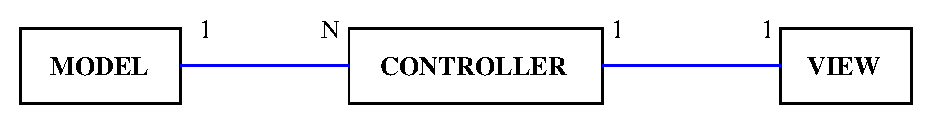
\includegraphics[width=10cm]{eps/mvc.eps}
\caption{\label{MVC_f}Simplified Model-View-Controller Pattern}
\end{center}
\end{figure}
Simplification consists in the fact that in the more general pattern
the Controller-View relationship allows a 1-N cardinality.
Furthermore, the implementation is different as the view side cannot
see the model part. The reasons behind this difference will be
explained later, but we can anticipate here that this is due to the
relationship between the view and the controller, that is stronger in
\pygtkmvc than in the classic \mvc.

\smallskip

Figure \ref{MVC_f} shows three interconnected parts:

\begin{description}
\item[Model] Contains the \emph{state} of the application. Also it
  provides support to access and modify the state, and knows how to
  handle dependencies between different parts in the state. For
  example the application logic could require that changing a
  variable, causes a changing of another. It is not required the
  model user to be aware about this dependency, because model
  autonomously handles it.

  Zero, one or more \emph{Controllers} can be connected to one Model
  (see \emph{Controller}, below). Furthermore, one or more
  \emph{Views} can be associated with parts of the state; for example
  a numerical variable could be visualized as a number, as well as a
  graphic bar. It is important to remark that \emph{a Model does not
    know that a set of Views is possibly connected to its state
    through a set of Controllers}.

\item[View] shows parts of the Model state, and interactively
  exchanges information with the User, via input/output devices.  View
  also interacts with a \emph{Controller} (see below), sending to it
  signals, and receiving information to visualize.

  Furthermore, a View collects a set of widget trees built from a
  \glade file, and/or constructed by hand. Since a Widget contains a
  \emph{state}, this implementation differs from the standard \mvc,
  where generally the View side is completely \emph{stateless}.

  As for the Model, a View does not know the semantics concerning what
  it visualizes, as well as the Model which it is connected to.

\item[Controller] Realizes the connection between Models and Views.
  A Controller contains the \gui logic: for example, it stores the
  information about what happens when a button is clicked (e.g. 
  handlers of signal are located inside a Controller.)

  A Controller perfectly knows how the connected Model and View are
  implemented, and knows both the state and presentation (\gui)
  semantics. A Controller is associated to one Model (\emph{has a}
  relationship), and in the current implementation is associated only
  to one View.

\end{description}


Two particular mechanisms make the isolation between Model and
Controller, and between View and Controller. To support the former,
the \obs is provided (see \ref{OBS}), whereas latter mechanism is
provided by the \mvc, and that is explained in \ref{VR}.


\subsubsection{\label{VR} View Registration}
Current implementation allows only a 1-1 relationship between
Controller and View. Anyway a registration mechanism has been provided
to connect those two parts, allowing for more generic relationship in
the future, when a Controller could handle more than one Views, or a
View can be shared among several Controllers.

After the creation, a View must register itself with a Controller.
From there on, the Controller can access the state (the set of
contained widgets) and methods inside the View. When the view
registers itself with a Controller, all signals are also automatically
connected to the corresponding methods inside the Controller.
Connection in this case is performed by means of an implicit syntax
rule, which binds a signal name to a corresponding method name.

In sections \ref{VR:D} and \ref{VR:EX} more details and an example are
presented, to show how the View registration mechanism can be
exploited by controllers to connect signals and handle the creation of
particular widgets like for example TreeViews, TreeColumns,
CellRenderers, etc.


\subsection{\label{OBS} Implementation of the \obs}

A Model does not know that it is connected to a set of controllers,
because this knowledge implies the knowledge of the \gui semantics,
which has to be out-of-scope for the Model.

Nevertheless, sometimes it is necessary for a Model to communicate to
the \gui logics (generally the Controllers set) that the model state
changed. This communication can be implemented by the \obs, that
provides a mechanism where \emph{Observers} are notified when
\emph{observed} state in the model get changed.

Even if models are typically observed by the \gui logics, the
mechanism can be used also to decouple (isolate) models and other
entities in the application logics. For example, models can be
observed by other models.

In \pygtkmvc Models' state has been extended with a mechanism called
\emph{Observable Properties}. An observable property is a part of the
Model state which is also externally observable via an
\emph{Observer}. Every time an observable property changes, any
interested Observer will be notified of the event.

Figure \ref{F:OBS} shows a Model (\kw{Model1}) containing an
observable property (\kw{color}). There are also a Controller and a
View (to show the colour), and the Controller is also an observer of
\kw{Model1}. Furthermore, there is another Observer that is model 
\kw{Model2}, whose state the designer wanted to make dependent on the
state of \kw{Model1}, but without explicitly coupling the two models.

When the property \kw{color} changes for example to red, all connected
Observers will be notified. Each observer will then perform the
necessary operation according to the respective logics. For example,
the Controller will make the connected View showing the occurred
change.

\begin{figure}[htbp]
\begin{center}
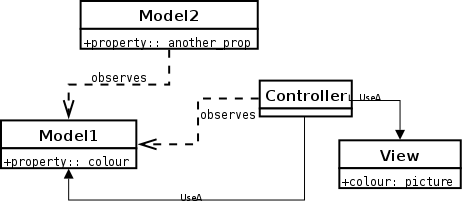
\includegraphics[width=10cm]{figs/png/obs.png}
\caption{\label{F:OBS}Observable models and Observers}
\end{center}
\end{figure}

Each Observer declares it is interested in receiving notifications on
one or more properties changing, by a mechanism called
\kw{Registration}. Once an Observer (for example, a Controller)
registered itself with the Model it is associated with, it will be
notified of all changes of the observable properties. The Observers
will be notified only of the property changes that they are actually
interested in observing.

An implicit syntactical rule binds observable property names to
notifications sockets inside Observers. This rule allows an automatic
connection, and fixes a sort of ``rule'' for methods names.

Later in this document, some implementation details are discussed, and
further details about observable properties are presented. Finally,
an example in the latest part should make all these concepts clearer.

\emph{Adapters} (see section \ref{ADAPT} are powerful entities that
can be used to automatically bind part of the view with part of the
model with a minimal effort, without any need to couple with complex
code and naming rules. However, \emph{Adapters} should be used only
after all the ``manual'' mechanisms have been well understood, and
for this reason they are presented only at the end of this document.


\subsubsection{\label{KOBS} Supported types of Observable Properties}

Observable properties can hold several types of values:

\begin{description}
\item [Any type] Change notification will occur only when the value is
  \emph{assigned} to the property.

\item [Mutable sequential types] Like lists and maps. A notification
  will occur when the \emph{content} of the object changes, e.g.
  when one element of the sequence is assigned, added, removed, etc.
 
\item [User classes] The user can declare the set of methods that can
  be observed (i.e. observables will be notified before and/or after
  observed object \emph{methods} are called.)

\item [Events] To notify the observers that some event is occurred.
\end{description}

All needed details about observable property types are explained later
in this document (see section \ref{KOBS:DET}).

% ----------------------------------------------------------------------

\newpage
% ----------------------------------------------------------------------
%%% Started on  Fri Dec 15 16:03:20 2006 Roberto Cavada
%%% Last Sat Dec 16 18:15:11 2006 Roberto Cavada

\section{\label{DI}Details of implementation}
This section presents some details regarding the implementation of the
\mvco framework in Python.

\subsection{Models, Controllers and Views in detail}
The \mvco framework essentially supplies three base classes which
implement respectively a View, a Model and a Controller.  Developers
have to derive custom classes from the base classes set, adding the
implementation which depends on the application semantics.

\begin{description}

\item[Model base class] Supplies servicing for:
 \begin{itemize} 
 \item Fully automatic Observable Properties 
 \item Automatic broadcast notification when observable properties
 change.
 \item Transparent notifications to observers running in the \pygtk
   loop, even when sent by models running from other threads.
 \end{itemize}

\item[Controller base class] Supplies servicing for:
 \begin{itemize} 
 \item Automatic registration as observers of the associated Model.
 \item Easy access to the associated Model and View for any derived
   class.
 \item Instantiation of \emph{adapters}.
 \end{itemize}

\item[View base class] Supplies servicing for:
 \begin{itemize} 
 \item Automatic widgets tree registration. Input can be a set of root
 widgets stored inside a \glade File, or a completely customized widgets
 hierarchies.
 \item Automatic signals connection to methods supplied by the
 associated Controller.
\item Widget retrieval inside the set of hierarchy. Widget can be
  accessed by using the name they have been defined from within
  \glade, at design time, or that have been specified when creating
  widgets by hand.
\item Support for custom widgets declared in \glade files.
 \end{itemize}

\end{description}


\subsection{\label{MODELS} Models}
Models must be used to hold the \emph{data} of the application. They
can be connected to observers (like Controllers) by a mechanism
detailed by section \ref{OPD}.  It is important to note that apart
from during the registration phase, the model does not know that
there exists a set observers connected to it.

All the code strictly related to the data of the application (i.e. not
related to any view of those data) will live in the model class. 

There exist several model classes that users can derive their own
classes:

\begin {description}
\item [gtkmvc.Model] Standard model class. The derived class does not
  multiple-derive from gobject classes, and there are not methods in
  the class that run from threads different from the \pygtk main loop
  thread. This is the base model class most likely users will derive
  their own models.

\item [gtkmvc.ModelMT] Multi-threading model used as the previous
  class Model, but to be used in all cases when the \pygtk main loop
  runs in a thread that is different from the thread running the
  model. This is the typical case of a model that needs to perform
  asynchronous operations that requires much time to complete, and
  that can be ran on a different thread making the \gui still
  responsive to the user actions. When the model's thread changes an
  observable property, corresponding notifications will be
  transparently delivered to the observers through their own thread.

\item [gtkmvc.TreeStoreModel] To be used as a base model class that
  derives both from \codename{Model} and \codename{gtk.TreeStore}.

\item [gtkmvc.TreeStoreModelMT] To be used as a base model class that
  derives both from \codename{ModelMT} and \codename{gtk.TreeStore}.

\item [gtkmvc.ListStoreModel] To be used as a base model class that
  derives both from \codename{Model} and \codename{gtk.ListStore}.

\item [gtkmvc.ListStoreModelMT] To be used as a base model class that
  derives both from \codename{ModelMT} and \codename{gtk.ListStore}. 

\item [gtkmvc.TextBufferModel] To be used as a base model class that
  derives both from \codename{Model} and \codename{gtk.TextBuffer}.

\item [gtkmvc.TextBufferModelMT] To be used as a base model class that
  derives both from \codename{ModelMT} and \codename{gtk.TextBuffer}.

\end{description}


\subsection{Controllers}
User's controllers must derive from this class.  A controller is
always associated with one model, that the controller can monitor and
modify. At the other side the controller can control a View.  Two
members called \codename{model} and \codename{view} hold the
corresponding instances.

The controller holds all the code that lives between data in model and
the data-presentation in the view. For example the controller will
read a property value from the model, and will send that value to the
view, to visualize it.  If the property in the model is an Observable
Property that the Controller is interested in monitoring, than when
somebody will change the property, the controller will be notified and
will update the view.


\subsubsection{Model registration}
By default, a controller is also an Observer (see below) of the
corresponding Model, even when there is nothing to observe, or when
the controller is interested in observing nothing within the model.

Registration occurs automatically. If the observation is not wanted,
the derived controller can call method \codename{unregister\_model}
from the instance constructor, to unregister itself.


\subsubsection{\label{VR:D}View registration}
View registration (see View class, below) occurs upon Controller
construction. An important method of the class Controller that user
can override is \codename{register\_view}, that the Controller will
call during View's registration. This can be used to connect custom
signals to widgets of the view, or to perform some initialization
that can be performed only when model, controller and view are
actually connected.  \codename{register\_view} gets the view
instance that is performing its registration within the
controller. See section \ref{VR:EX} for an example of how this
mechanism may be exploited effectively.

\subsection{Views}
User's views derive from base class \codename{gtkmvc.View}, that is
the only part specific for the \pygtk graphic toolkit.

A View is associated to a set of widgets. In general, this set
can be organized as a set of trees of widgets. Each tree can be
optionally be generated by using the \glade application 
(see section \ref{GLEX}). 


\subsubsection{Constructor}

The View constructor is quite much complicated:

{ \codesize 
\begin{verbatim} 
def __init__(self, glade=None, top=None, parent=None)
\end{verbatim}} 


\begin{description}
\item[glade] can be either a string or a list of strings. In
  any case each provided string represents the file name of a \glade
  file. Typically each glade file contains a tree of (named) widgets.
   
  When not given (of \codename{None}) a corresponding class member
  called \codename{glade} is checked. If also \codename{self.glade}
  is \codename{None} it means that there is no \glade file and the
  widgets will have to be constructed manually.
  
\item[top] can be a string or a list of strings.  Each string
  provided is associated to the parameter \codename{glade} content,
  and represent the name of the widget in the widgets tree
  hierarchy to be considered as top level. This lets the user to
  select single parts of the glade trees passed through parameter
  \codename{glade}. 

  When not given (of \codename{None}) a corresponding class member
  called \codename{top} is checked. If also \codename{self.top} is
  \codename{None} it means that the root widget name of the given
  \glade file will be taken as the name for the top level widget.

\item[parent] is the view instance to be considered parent of
  self. This can be used in special cases to construct hiearchical
  views. Generally this parameter is None or not given.

\end{description}


\subsubsection{\label{VIEW:MANUAL}A widgets container}

The \codename{View} class can also be considered a map, that
associates widget names to the corresponding widget objects. If file
\file{test.glade} contains a Button that you called
\codename{start\_button} from within \glade, you can create the view
and use it as follows:

{ \codesize 
\begin{verbatim}
from gtkmvc import View

class MyView (View):
  glade = 'test.glade'
  pass 

m = MyModel()
v = MyView()
c = MyController(m, v)

v['start_button'] # this returns a gtk.Button object
\end{verbatim}
}

Instead of using only \glade files, sometimes the derived views create
a set of widgets on the fly. If these widgets must be accessed later,
they can be associated simply by (continuing the code above):

{ \codesize 
\begin{verbatim}
v['vbox_widget'] = gtk.VBox()
...
\end{verbatim}
}

The creation on the fly of new widgets should be performed within
the derived view cosntructor:

{ \codesize 
\begin{verbatim}
from gtkmvc import View

class MyView (View):
  def __init__(self, ):
    super(MyView, self).__init__('test.glade')

    self['vbox_widget'] = gtk.VBox()
    ...
    return

  pass 
\end{verbatim}
}


Another important mechanism provided by the class View is the signals
auto-connection. By using \glade users can associate to widget's
signals functions and methods to be called when associated events
happen.  When performs the registration, the View searches inside the
corresponding Controller instance for methods to associate with
signals, and all methods found are automatically connected.


\subsubsection{Custom widgets support}
A basic support for Custom widgets is provided since version 1.0.1.
Designers can specify custom widgets within a \glade file, and for
each custom widget they may specify a function name to be called to
build it. The specified function will be searched and invoked among
the \codename{View} methods when the instance is
created. \codename{View}'s method for custom widget creation
has prototype:

{ \codesize 
\begin{verbatim}
 def func_name(self, str1, str2, int1, int2)
\end{verbatim}
}

Creation functions are expected to return a widget object.


\subsubsection{\label{VR:EX}An example about View Registration}
A typical example of exploitation of the view registration mechanism
is the setup of a \codename{gtk.TreeView} chain: construction of
\codename{TreeView}, \codename{TreeViewColumn},
\codename{CellRenderers}, connection to the \codename{TreeModel}, etc.
As \glade does not provide a full support for these widgets, and as
the \codename{TreeModel} lives in the model-side of the application,
their construction cannot occur within the View, but must be performed
within the Controller, that knows both the view and model sides. The
right time when this construction has to occur is the view
registration.

The idea is to have a \codename{TreeView} showing an integer and a
string in two separated columns from a \codename{gtk.ListStore}.  

Now suppose you created a project in \glade that contains a window,
some menus and other accessories, and a \codename{TreeView} whose
properties are set in \glade in a comfortable manner (see figure
\ref{fig:VR}).

\begin{figure}[here]
\begin{center}
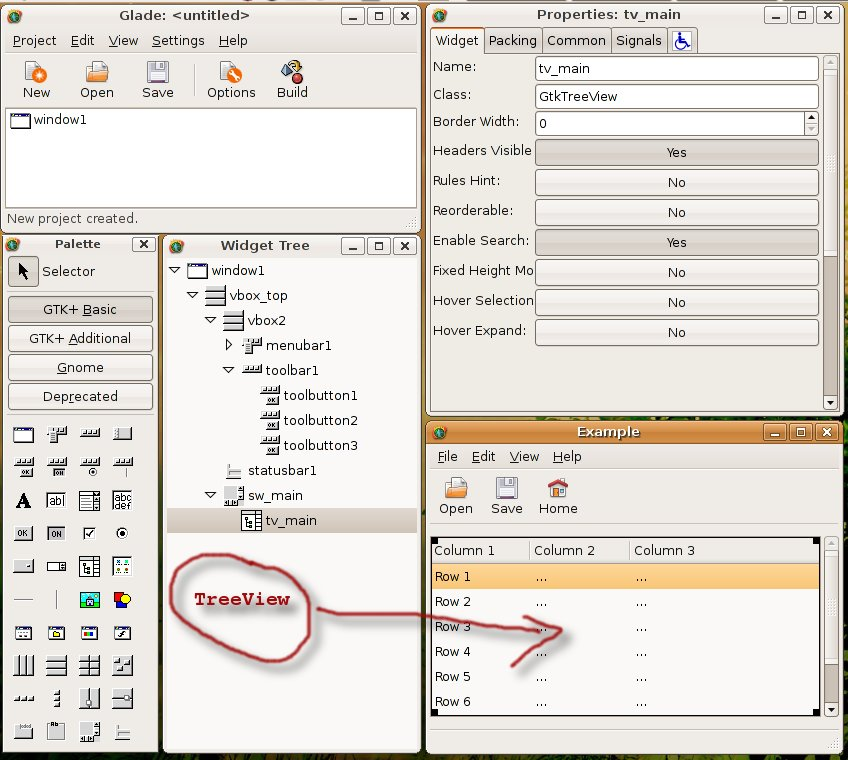
\includegraphics[width=12cm]{figs/png/treeview}
\caption{\label{fig:VR}Designing a \codename{TreeView} by means of \glade }
\end{center}
\end{figure}

In the example, the \codename{TreeView} has been called
\codename{tv\_main}, and after View creation the widget will be
available with that name.

{ \codesize 
\begin{verbatim}
from gtkmvc import View

class MyView (View):
  def __init__(self):
    super(MyView, self).__init__('test.glade')
    #...
    return
  pass 
\end{verbatim}
}

The \codename{ListStore} is of course not contained in the view, but
it is created and stored in the Model. If the model had to be also a
\codename{ListStore} (i.e.  derived from it) \codename{MyModel} had to
derive from \codename{gtkmvc.ListStoreModel} instead of
\codename{Model}. To keep things easier, Has--A relationship is
chosen.

{ \codesize 
\begin{verbatim}
from gtkmvc import Model
import gtk
import gobject

class MyModel (Model):
  def __init__(self):
    Model.__init__(self)

    self.list = gtk.ListStore(gobject.TYPE_INT, gobject.TYPE_STRING)
    return
  pass 
\end{verbatim}
}

The controller has the responsibility of connecting the
\codename{TreeView} and the \codename{ListStore}, and it creates
columns and renderers as well. Construction must occur after View has
been created. More precisely, the ideal time is during
view-registration.

{ \codesize 
\begin{verbatim}
from gtkmvc import Controller
import gtk

class MyCtrl (Controller):

  def register_view(self, view):
    tv = self.view['tv_main']    
    tv.set_model(self.model.list) # sets the model

    # creates the columns
    cell = gtk.CellRendererText()
    col = gtk.TreeViewColumn('Int', cell, text=0)
    tv.append_column(col)

    cell = gtk.CellRendererText()
    col = gtk.TreeViewColumn('String', cell, text=1)
    tv.append_column(col)

    # registers any treeview-related signals...
    return

  pass # end of class 
\end{verbatim}
}



\subsection{\label{OPD}Observable Properties in details}
The mechanism of the Observable Properties (\OP) is fully automatic,
since its management is carried out by the base class
\codename{Model}.

Basically the user derives from class \codename{Model} (or the others
listed in section \ref{MODELS}). The user adds a class variable
called \OPvar. This variable must be a map, whose elements' keys are
names of properties, and the associated values are the initial values.

For example, suppose you want to create an \OP called \codename{name} 
initially associated to the string value ``Rob'':

{ \codesize 
\begin{verbatim} 
from gtkmvc import Model

class MyModel (Model):
  __properties__ = { 'name' : 'Rob' }

  def __init__(self):
    Model.__init__(self)
    # ...
    return

  pass # end of class
\end{verbatim}
}

By using a specific meta-class, property \codename{name} will be
automatically added, as well as all the code to handle it.

This means that you may use the property in this way:
{ \codesize 
\begin{verbatim} 
m = MyModel()
print m.name  # prints 'Rob'
m.name = 'Roberto' # changes the property value
\end{verbatim}
}

What's missing is now an observer, to be notified when the property
changes. To create an observer, derive your class from base class
\codename{gtkmvc.Observer}.

{ \codesize 
\begin{verbatim} 
from gtkmvc import Observer

class AnObserver (Observer):
  def __init__(self, model):
    Observer.__init__(self, model)

    # ...
    return

  def property_name_value_change(self, model, old, new):
    print ``Property name changed from '%s' to '%s''' % (old, new)
    return

  pass # end of class
\end{verbatim}
}

The Observer constructor gets an instance of a Model, and registers the
class instance itself to the given model, to become an observer of
that model instance.

To receive notifications for the property \codename{name}, the
observer must define a method called
\codename{property\_name\_value\_change} that when is automatically
called will get the instance of the model containing the changed
property, and the property's old and new values.

As already mentioned, when used in combination with the \mvc,
Controllers are also Observers of their models.

Here follows an example of usage:
{ \codesize 
\begin{verbatim} 
m = MyModel()
o = AnObserver(m)

print m.name  # prints 'Rob'
m.name = 'Roberto' # changes the property value, o is notified
\end{verbatim}
}

Things so far are easy enough, but they get a bit complicated when you
derive custom models from other custom models.  For example, what
happens to \OP if you derive a new model class from the class
\codename{MyModel}?

In this case the behavior of the \OP trusty follows the typical Object
Oriented rules:
\begin{enumerate}
    \item Any \OP in base class are inherited by derived classes.
    \item Derived class can override any \OP in base classes.
    \item If multiple base classes defines the same \OP, only the
      first \OP will be accessible from the derived class.
\end{enumerate}

For example:

{ \codesize
\begin{verbatim} 
from gtkmvc import Model

class Test1 (Model):
    __properties__ = {
        'prop1'  : 1
        }

    def __init__(self):
        Model.__init__(self)

        # this class is an observer of its own properties:
        self.register_observer(self) 
        return
    
    def property_prop1_value_change(self, model, old, new):
        print "prop1 changed from '%s' to '%s'" % (old, new)
        return
    pass # end of class

class Test2 (Test1):    
    __properties__ = {
        'prop2'  : 2,
        'prop1'  : 3
        }
    
    def __init__(self):
        Test1.__init__(self)
        
        # also this class is an observer of itself:
        self.register_observer(self)
        return
    
    def property_prop2_value_change(self, model, old, new):
        print "prop2 changed from '%s' to '%s'" % (old, new)
        return
    pass

# test code:
t1 = Test1()
t2 = Test2()

t2.prop2 = 20
t2.prop1 = 30
t1.prop1 = 10
\end{verbatim}
}

When executed, this script generates this output:
{ \codesize 
\begin{verbatim} 
prop2 changed from '2' to '20'
prop1 changed from '3' to '30'
prop1 changed from '1' to '10'
\end{verbatim}
}

As you can see, \codename{t2.prop1} overrides the \OP \codename{prop1}
defined in Test1 (they have different initial values).  Test2 could
also override method \codename{property\_prop1\_value\_change}:

{ \codesize 
\begin{verbatim} 
class Test2 (Test1):
  # ... copy from previous definition, and add:
   
  def property_prop1_value_change(self, model, old, new):
    print "Test2: prop1 changed from '%s' to '%s'" % (old, new)
    return   

  pass
\end{verbatim}
}

As you expect, the output in this case would be:
{ \codesize 
\begin{verbatim} 
prop2 changed from '2' to '20'
Test2: prop1 changed from '3' to '30'
prop1 changed from '1' to '10'
\end{verbatim}
}


\subsubsection{\label{KOBS:DET}Types of Observable Properties}

In section \ref{KOBS} we anticipated that there exist several types
of \OP. In the examples so far we have seen only \emph{value} \OPS,
meaning that observers will be notified of any change of \emph{value}
assigned to the corresponding \OP. What would happen if the value of
the property would be a complex object like a list, or a user-defined
class, and the object would change internally?

For example:

{ \codesize 
\begin{verbatim} 
from gtkmvc import Model

class MyModel (Model):
    __properties__ = {
        'prop1'  : [1,2,3]
        }

    def __init__(self):
        Model.__init__(self)
        ...
        return
    pass # end of class

m = MyModel()
m.prop1.append(4)
m.prop1[1] = 5
\end{verbatim}
}

Last two lines of the previous example actually change the \OP
internally, that is different from \emph{assigning} a new value to the
property like in \verb@m.prop1 = [5,4,3,2]@ that would trigger a value
notifications like those seen in previous examples.  Similar problem
is found when the property is assigned to a class instance, and then a
method that change the instance is called.

\emph{Mutable sequential types} and \emph{User classes} are also
supported by the \obs of \pygtkmvc, but the name of the notified
method in the controller has to be changed accordingly.
The idea is to provide two methods to be notified:
\begin{description}
\item[property\_\codename{name}\_before\_change] That is called
  immediately \emph{before} a method that changes the instance is
  called on the \OP called \codename{name}.
\item[property\_\codename{name}\_after\_change] That is called
  immediately \emph{after} a method that changes the instance is
  called on the \OP called \codename{name}.
\end{description}

Of course, it is not needed to define both of the two methods in the
observer class, as only the actually defined methods will be called. 

The signature of these methods is:
{ \codesize 
\begin{verbatim} 
    def property_<name>_before_change(self, model, instance, name,
                                      args, kwargs)

    def property_<name>_after_change(self, model, instance, name, 
                                     res, args, kwargs)
\end{verbatim}
}

\begin{description}
\item[self] The Observer class instance defining the method.
\item[model] The Model instance containing the \OP called
  \verb@<name>@ that is being changed.
\item[instance] The object instance that is assigned to the \OP called
  \verb@<name>@.
\item[name] The name of the method that is being called. This
  is different from \verb@<name>@ that is the name of the \OP
  contained in the model. 
\item[res] (Only for \emph{after} notification) the value returned by
  the method \emph{name} that has been called on the \OP
  \emph{instance}.
\item[args] List of arguments of the method \emph{name}.
\item[kwargs] Map of keyword arguments of the method \emph{name}.
\end{description}

As it can be noticed, the only difference between these two method
signatures is the parameter \emph{res} that is obviously available only
for notification method \emph{after}.

The framework \mvco provides a full support for python mutable
sequences like \kw{lists} and \emph{maps}. For example:


{ \codesize 
\begin{verbatim} 
from gtkmvc import Model, Observer

# ----------------------------------------------------------------------
class MyModel (Model):    
    __properties__ = {
        'myint'  : 0, 
        'mylist' : [],
        'mymap'  : {},
        }

    pass # end of class

# ----------------------------------------------------------------------
class MyObserver (Observer):

    # notifications

    def property_myint_value_change(self, model, old, new):
        print "myint changed"
        return

    def property_mylist_value_change(self, model, old, new):
        print "mylist changed"
        return

    def property_mylist_before_change(self, model, instance, name,
                                      args, kwargs):
        print "mylist before change:", instance, name, args, kwargs
        return

    def property_mylist_after_change(self, model, instance, name, res,
                                     args, kwargs):
        print "mylist after change:", instance, name, res, args, kwargs
        return

    # for mymap value_change and before_change are not provided!
    def property_mymap_after_change(self, model, instance, name, res,
                                    args, kwargs):
        print "mymap after change:", instance, name, res, args, kwargs
        return

    pass # end of class


# Look at what happens to the observer
if __name__ == "__main__":

    m = MyModel()
    c = MyObserver(m)

    # changes the int:
    m.myint = 20

    # changes the list:
    m.mylist = [1,2]             # calls value_change
    m.mylist.append(10)     
    m.mylist[0] = m.mylist[0]+1

    # changes the map:
    m.mymap["hello"] = 30
    m.mymap.update({'bye' : 50})
    del m.mymap["hello"]
    pass
\end{verbatim}
}

After the execution, this is the program output:

{ \codesize 
\begin{verbatim} 
myint changed
mylist changed
mylist before change: [1, 2] append (10,) {}
mylist after change: [1, 2, 10] append None (10,) {}
mylist before change: [1, 2, 10] __setitem__ (0, 2) {}
mylist after change: [2, 2, 10] None __setitem__ (0, 2) {}
mymap after change: {'hello': 30} None __setitem__ ('hello', 30) {}
mymap after change: {'bye': 50, 'hello': 30} update None ({'bye': 50},) {}
mymap after change: {'bye': 50} None __delitem__ ('hello',) {}
\end{verbatim}
}

This covers those cases where you have your \OPS holding mutable
sequence values. What if the value is a user-defined class instance?
The notification mechanism is the same: when a method \codename{M}
that changes internally the instance is called, Observer's methods
\kw{before} and \kw{after} will be called. However, how can the user
declare that method \codename{M} \emph{does changes} the instance?
Two mechanism are provided by the framework:
\begin{itemize}
\item For already existing classes and class instances. In this cases
  the declaration occurs when the instance is assigned to the \OP in
  the model.
\item For ad-hoc and new classes. In this case the method will be
  \emph{declared} as \kw{Observable} at the class level, through a
  special \kw{decorator} provided by the framework. This is the
  preferable manner. 
\end{itemize}

Examples for new classes:

{ \codesize 
\begin{verbatim} 
from gtkmvc import Model
from gtkmvc import Observer
from gtkmvc import observable

# ----------------------------------------------------------------------
class AdHocClass (observable.Observable):
    def __init__(self): self.val = 0

    # this way the method is declared as 'observed':
    @observable.observed 
    def change(self): self.val += 1

    # this is NOT observed:
    def is_val(self, val): return self.val == val

    pass #end of class

# ----------------------------------------------------------------------
class MyModel (Model):
    __properties__ = {
        'obj' : AdHocClass(),
        }

    def __init__(self):
        Model.__init__(self)
        return    

    pass # end of class

# ----------------------------------------------------------------------
class MyObserver (Observer):
    def __init__(self, model):
        Observer.__init__(self, model)
        return

    def property_obj_value_change(self, model, old, new):
        print "obj value changed from:", old, "to:", new 
        return

    def property_obj_after_change(self, model, instance, name, res,
                                  args, kwargs):
        print "obj after change:", instance, name, res, args, kwargs
        return

    pass

# Look at what happens to the observer
if __name__ == "__main__":
    m = MyModel()
    c = MyObserver(m)
    m.obj.change()
    m.obj = None
    pass
\end{verbatim}
}

The execution prints out (slightly modified for the sake of
readability):

{ \codesize 
\begin{verbatim} 
obj after change: <__main__.AdHocClass object at 0xb7d91e8c> 
change None (<__main__.AdHocClass object at 0xb7d91e8c>,) {}

obj value changed 
from: <__main__.AdHocClass object at 0xb7d91e8c> to: None
\end{verbatim}
}

As you can see, declaring a class as \emph{observable} is as simple as
deriving from \codename{gtkmvc.observable.Observable} and decorating
those class methods that must be observed with the decorator 
\codename{gtkmvc.observable.observe} (decorators are supported by
Python version 2.4 and later only). 

\vspace{4mm}
What if the user class cannot be easy changed, or only an instance of
the class is available as \OP value? In this case declaration of the
methods to be observed can be done at time of declaration of the
corresponding \OP. In this case the \emph{value} to be assigned to the
\OP must be a triple \verb@(class, instance, method_names>@, where:
\begin{description}
\item[class] Is the \codename{class} of the object to be observed.
\item[instance] Is the object to be observed.
\item[method\_names] Is a tuple of strings, representing the method
  names of the instance to be observed.
\end{description}

For example:
{ \codesize 
\begin{verbatim} 
from gtkmvc import Model

#----------------------------------------------------------------------
# This is a class the used cannot/don't want to change
class HolyClass (object):    
    def __init__(self): self.val = 0 
    def change(self): self.val += 1
    pass #end of class


# ----------------------------------------------------------------------
class MyModel (Model):

    __properties__ = {
        'obj' : (HolyClass, HolyClass(), ('change',)),
        }

    def __init__(self):
        Model.__init__(self)
        return    

    pass # end of class
\end{verbatim}
}



\vspace{4mm}
Finally, \OP can hold special values that are \kw{signals} that can be
used to notify observers that certain events occurred. 

To declare an \OP as a signal, the value of the \OP must be
\codename{gtkmvc.observable.Signal()}. To notify an event, the model
can then invoke method \codename{emit} of the \OP. The observers will
be notified by calling method
\codename{property\_<name>\_signal\_emit} that will also receive any
parameter passed to the \codename{emit} method. For example:

{ \codesize 
\begin{verbatim} 
from gtkmvc import Model
from gtkmvc import Observer
from gtkmvc import observable

# ----------------------------------------------------------------------
class MyModel (Model):
    __properties__ = {
        'sgn'  : observable.Signal(),
        }

    def __init__(self):
        Model.__init__(self)
        return    
    pass

# ----------------------------------------------------------------------
class MyObserver (Observer):
    def __init__(self, model):
        Observer.__init__(self, model)
        return

    # notification
    def property_sgn_signal_emit(self, model, args, kwargs):
        print "Signal:", model, args, kwargs
        return

    pass # end of class

# Look at what happens to the observer
if __name__ == "__main__":
    m = MyModel()
    c = MyObserver(m)
    m.sgn.emit() # we emit a signal
    m.sgn.emit("hello!", key=10) # with arguments
    pass
\end{verbatim}
}

The execution of this example will produce:

{ \codesize 
\begin{verbatim} 
Signal: <__main__.MyModel object at 0xb7de564c> () {}
Signal: <__main__.MyModel object at 0xb7de564c> ('hello!',) {'key': 10}
\end{verbatim}
}

In the \file{examples}, there are several examples that show how
different types of \OPS can be used. Of course all available types can
be used in all available kind of model classes, with or without
multi-threading support.

  
\subsubsection{Special members for Observable Properties}
Classes derived from Model, that exports \OPS, have several special
members. Advanced users might be interested in overriding some of them,
but in general they should be considered as private members. They are
explained here for the sake of completeness.

\begin{description}

\item[\OPvar] A class (static) member that maps property names and
initial values. This must be provided as a map by the user.

\item[\OPdvar] Automatically generated static member that maps the 
\OPS exported by all base classes. This does not contain \OPS that 
the class overrides. 

\item[\codename{\_prop\_\emph{property\_name}}] This is an
  auto-generated variable to hold the property value. For example, a
  property called \codename{x} will generate a variable called
  \codename{\_prop\_x}.

\item[\codename{get\_prop\_\emph{property\_name}}] This public method
  is the getter for the property. It is automatically generated only
  if the user does not define one. This means that the user can change
  the behavior of it by defining their own method.  For example, for
  property \codename{x} the method is \codename{get\_prop\_x}.  This
  method gets only self and returns the corresponding property value.

\item[\codename{set\_prop\_\emph{property\_name}}] This public method
  is customizable like \\
  \codename{get\_prop\_<property\_name>}.  This does not return
  anything, and gets self and the value to be assigned to the
  property. The default auto-generated code also calls method
  \codename{gtkmvc.Model.notify\_property\_change} to notify the
  change to all registered observers.

\end{description}

For further details about this topic see meta-classes \codename{PropertyMeta}
and \\
\codename{ObservablePropertyMeta} from package \codename{support}.



% ----------------------------------------------------------------------

\newpage
% ----------------------------------------------------------------------
%%
%% exam.tex
%% 
%% Made by Roberto Cavada
%% Login   <cavada@localhost.localdomain>
%% 
%% Started on  Sat Dec 16 18:18:21 2006 Roberto Cavada
%% Last on Sat Dec 16 18:26:47 2006 Roberto Cavada
%%


\section{\label{SAP} A simple application}
This section describes the process of creation of a sample
application, from the design with \glade, to the integration of views
and code inside the \mvco Infrastructure.

We want to design and implement a simple application constituted by
only one window, containing two string labels. One label shows a text,
while the other shows the number of characters displayed (i.e. the
length of the string) by the first one. There is also a button the
user can press. By pressing the button, the user can change the
displayed text, and of course this action might change also the
displayed text length accordingly. Figure \ref{EX:f} gives an idea on
how the application should appear.

\begin{figure}[htbp]
\begin{center}
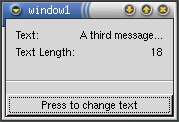
\includegraphics[width=4cm]{figs/png/example}
\caption{\label{EX:f}The sample Application}
\end{center}
\end{figure}

\subsection{\label{GLEX}\glade}
Figure \ref{GL:f} shows \glade and a project named \codename{example}.
The sample \gui has only one top-level window (named
\codename{window1}).

\begin{figure}[here]
\begin{center}
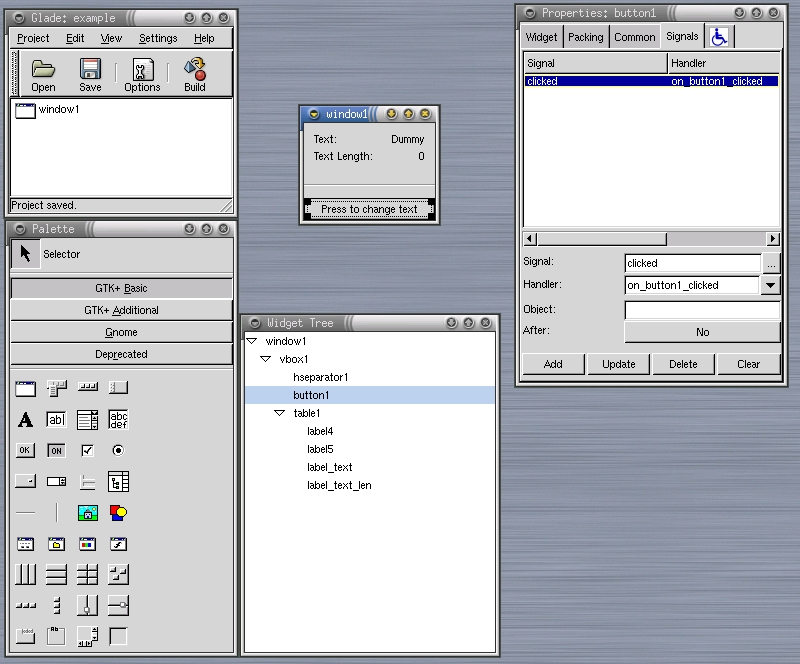
\includegraphics[width=12cm]{figs/png/example_glade}
\caption{\label{GL:f}Designing the example by means of \glade for GTK2}
\end{center}
\end{figure}

The \appl{Widget Tree Window} shows the widgets hierarchy. There are
essentially the three main components (one button and two labels),
grouped inside a set of \emph{containers}, which supplies alignments and
resizing capabilities.

On the right side of Figure \ref{GL:f}, the \appl{Properties Window}
shows that the widget named \codename{button1} has signal
\codename{clicked} associated with function
\codename{on\_button1\_clicked}. This means that the Controller will
have to supply this function in order to handle the \codename{click}
event occurring in \codename{button1}.

\subsection{Implementation}
The implementation is slightly elaborate for this example, because the
goal here is to show how the sample application can be implemented by
using the \mvco Infrastructure.

A basic knowledge of any Object Oriented programming language is
sufficient to understand how this example has been pushed inside the
\mvco framework. On the contrary, a fair knowledge of the Python
language is required in order to understand the code details.

More description section is \ref{DI}.


\subsubsection{View}
In the example, the View is implemented inside the class
\codename{ExampleView} shown below.

{ \codesize 
\begin{verbatim}  
from gtkmvc import View
import os.path

GLADE_PATH = "./glade" 

class ExampleView (View):
    """The application view. Contains only the main window1 tree."""
    glade = os.path.join(GLADE_PATH, "example.glade")
    top = "window1"
    pass # end of class
\end{verbatim}}

Class \codename{ExampleView} extends the generic \codename{View}
class, which performs most of the job, as described above.
Class memebers \codename{glade} and \codename{top} are used instead of 
calling \codename{View} constructor directly. 

\subsubsection{Model}
Class \codename{ExampleModel} is as simple as class
\codename{ExampleView}.  As for \codename{ExampleView}, it extends a
base class of the \mvco Infrastructure, class \codename{Model}.  The
state is represented by a set of possible messages, as well as by the
current message index. The current message index is also an
observable property. A couple of methods are supplied in order to
access the state.

{ \codesize 
\begin{verbatim} 
from gtkmvc import Model

class ExampleModel (Model):
    """The model contains a set of messages
    and an observable property that represent the current message
    index"""

    # Observable property: code for that is automatically generated
    # by metaclass constructor. The controller will be the observer
    # for this property
    message_index = -1   # -1 is the initial value
    __observables__ = ("message_index",)

    def __init__(self):
        Model.__init__(self)

        self.messages= ('Initial message',
                        'Another message', 
                        'Another message again',
                        'Model changed again!')
        return

    def get_message(self, index): return self.messages[index]

    def set_next_message(self):
        # this changes the observable property:
        self.message_index = (self.message_index + 1) % len(self.messages)
        return

    pass # end of class

\end{verbatim}
}

Notice that class instance members are declared to be observable
through the special class variable \codename{\_\_observables\_\_},
which is a list of names (string) of the properties that are
observable.

The base class Model belongs to a
meta-class which automatically searches for observable properties and
generates the needed code to handle the notification.  When the value
of variable \codename{message\_index} changes, all registered
observers will be notified.

It is also possible to use the special class' variable
\codename{\_\_properties\_\_}, which is a map of (property, value)
couples. This variable was used in older versions of \gtkmvc and
now should be avoided.

\subsubsection{Controller}
Class \codename{ExampleController} contains the \emph{logic} of the
application. The controller handles two signals and the observable
property notification. Signals are the \codename{destroy} event,
invoked when the application quits, and the
\codename{on\_button1\_clicked}, fired when \codename{button1} is
pressed.

{ \codesize 
\begin{verbatim} 
from gtkmvc import Controller
from gtk import mainquit

class ExampleController(Controller):
    """The only one controller. Handles the button clicked signal, and
    notifications about one observable property."""

    def __init__(self, model, view):
        """Contructor. model will be accessible via the member 'self.model'.
        View registration is also performed."""
        Controller.__init__(self, model, view)
        return

    def register_view(self, view):
        # Connects the exiting signal:
        view.get_top_widget().connect("destroy", mainquit)
        return

    # Signal
    def on_button1_clicked(self, button):
        """Handles the signal clicked for button1. Changes the model."""
        self.model.set_next_message()
        return

    # Observables notifications (value):
    def property_message_index_value_change(self, model, old, new):
        """The model is changed and the view must be updated"""
        msg = self.model.get_message(new)
        
        self.view['label_text'].set_text(msg)
        self.view['label_text_len'].set_text(str(len(msg)))
        return    

    pass # end of class
\end{verbatim}
}

The \codename{destroy} signal is connected when the View registers
itself inside the controller, by using the method override of
\codename{register\_view}.  Method \codename{on\_button1\_clicked}
calls a method inside the model which changes a part of the state
inside the model. Since that part of the state is an observable
property, the associated observer (which is the controller itself) is
notified of the modification, by calling method
\codename{property\_message\_index\_value\_change}. This method
updates the view connected to the controller.


% ----------------------------------------------------------------------

\newpage
% ----------------------------------------------------------------------
\section {Adapters}
\label{ADAPT}

Version 1.2 introduces \emph{Adapters}, a powerful feature that
makes the framework perform some standard and boring activities
autonomously.

\subsection{Introduction}

Previous sections presented the framework and its main feature, that
is -- to recap it once again -- to provide a full support for
separating the logical and the presentation sides of an
application. This separation is featured by the \mvc and the \obs.

Although features are important, \emph{goals} are the driving
targets that lead the framework development. Most important goals of
the framework are to keep simplicity, transparency and lightness,
and to bear the level of abstraction high whilst still allowing to
control and customise lower levels.

It is the case that the framework forces and helps to both design
and implement applications in a clean and robust way. 

However, sometimes things get complicated even for simple
designs. In particular \kw{Controllers} tend to blow up in size and
complexity when handling a \kw{View} containing many widgets, and
when observing many properties into the \kw{Model}. Also, since the
framework can handle several kinds of observable properties (\OPS),
developers are required to remember and use some naming conventions
for notifications methods defined inside \kw{Observers}. Conventions
contributes to make things that would be easy too complex.

In particular, when a default behaviour is expected, the
\kw{Controller} gets filled in with many methods whose code follows
a template that is identically repeated all over again.

\bigskip 

For example, let us suppose it is needed to have a text entry always
aligned with some part of the model. This would require to have a
textual observable property into the model, a signal handler into
the controller to handle the \codename{'changed'} signal, and a
method to handle notification for observable property value
changes. When a \codename{'changed'} signal arrives, the
corresponding signal handler should read the text entry value and
report it to the observable property into the model. Viceversa, when
the observable property in the model get changed for any reason, the
notification code into the controller should update the text entry
value. The handlers' code should also avoid to fall into a
reciprocal loop.

\smallskip
It is in this context that adapters become pretty nifty. 

\subsection{What are Adapters}

\kw{Adapters} are the generalization of the the code that handles
autonomously the connection between a set of widgets and a
corresponding set of properties (possibly observable) to keep
aligned automatically the logical and the presentation sides, and to
keep low the complexity of controllers.

\begin{figure}[htbp]
\begin{center}
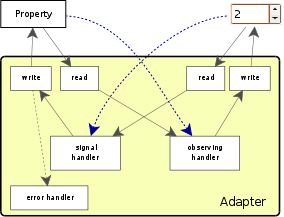
\includegraphics[width=10cm]{figs/png/adap}
\caption{\label{ADAP_f} Schematic simple adapter}
\end{center}
\end{figure}

In figure \ref{ADAP_f} is represented a simple adapter, where main
internal functional blocks are shown. There exist functional blocks
to control (and possibly customise) the way the property and the
widget are read and written. Also, there is a functional block to
manage how errors are handled when exceptions occur when writing
into the property.

An Adapter \emph{adapts} widgets and model's properties. Adapters
offer strong customization, but in their simplest use they are
pretty easy to be used. In this context, previous example might be
handled as follows.

We have a hand-made View containing a button and a text
entry. Notice that the name of the text entry is
\codename{entry\_text}.

{ \codesize
\begin{verbatim}
class MyView (gtkmvc.View):
    def __init__(self):
        super(MyView, self).__init__()

        w = gtk.Window(); e = gtk.Entry(); b = gtk.Button("Press")
        h = gtk.VBox(); h.add(e); h.add(b); w.add(h)
        w.show_all()
        self['entry_text'] = e
        self['button'] = b        
        return

    pass # end of class
\end{verbatim}
}


The model contains an observable property that should always 
reflect the content of the text entry \codename{entry\_text}.

{ \codesize
\begin{verbatim}
class MyModel (gtkmvc.Model):
    __properties__ = {
        'text' : "Ciao",
        }
    pass # end of class
\end{verbatim}
}

As usual, the controller is the most complex part, but by exploiting
an adapter it gets pretty much simplified. 
{ \codesize
\begin{verbatim}
class MyCtrl (gtkmvc.Controller):
    def register_adapters(self):
        self.adapt("text")
        return

    def register_view(self, view):
        view['button'].connect('clicked', self.on_button_clicked)
        return

    # signal handles
    def on_button_clicked(self, button):
        print "Text is:'%s'" % self.model.text
        return

    pass # end of class
\end{verbatim}
}

The idea in this example is to have ``\codename{button}''
that when pressed makes model's observable property \codename{text}
printed out to the standard output.

No code is included to handle \codename{entry\_text} ``change''
signal and observable property value change notifications. Instead,
a new method surfaces off the controller:
\codename{register\_adapters}.

This method is called at the right time by the framework and it is a
good place where adapters can be created and connected. In the
example, creation occurs through a call to another new method of
class Controller: \codename{adapt}. 

The new method is pretty complex and will be discussed in depth
later. Enough to say now that parameter \codename{"text"}
represents the name of the observable property that we want to
adapt. The corresponding widget is searched among all widgets in the
view, and widget \codename{entry\_text} is found and connected
automatically. The way this magic happens is not important at this
stage, but soon you will introduced with all details, to make you
know how to fully exploit and control this new feature.

\begin{figure}[htbp]
\begin{center}
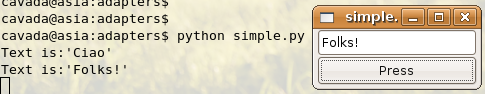
\includegraphics[width=10cm]{figs/png/adap1}
\caption{\label{ADAP1_f} Simple adapter at work}
\end{center}
\end{figure}


The code that instantiates and runs this example is as usual:
{ \codesize
\begin{verbatim}
m = MyModel()
v = MyView()
c = MyCtrl(m,v)
gtk.main()
\end{verbatim}
}

File \file{examples/adapters/simple.py} contains the full source
code of this example. When being run, it shows up a window
containing the text entry and the button. When the button is
pressed, the content of the observable property \codename{text} is
printed to the standard output. Initially, \codename{text} is
assigned to \codename{"Ciao"} and the text entry reflects it
accordingly.

If the user changes the text in the entry, the property
\codename{text} will be changed accordingly, as it is easy to check
by clicking the button. Viceversa, if the property \codename{text}
were changed by another model, observer, etc., the text entry would
get updated accordingly.


\subsection{Module \codename{adapters}}
Currently, module \codename{adapters} contains a few adapters
classes.

\begin{description}
\item [\codename{Adapter}] Connects a widget and a property. The
  property cannot be a container or a user-defined class.

\item [\codename{UserClassAdapter}] This class handles the
  communication between a widget and a class instance that is a
  property inside the model.

\item [\codename{RoUserClassAdapter}] This is similar to
  \codename{UserClassAdapter}, but dedicated to read-only class
  instances. Used internally to handle for example
  \codename{datetime} properties, when connecting a
  \codename{gtk.Calendar}.

\item [\codename{StaticContainerAdapter}] This class can be used to
  bound a set of widgets to a single property that is a container,
  like a tuple, a list or a map, or in general a class that
  implements \codename{\_\_getitem\_\_} and
  \codename{\_\_setitem\_\_} methods.
\end{description}


\begin{figure}[here]
\begin{center}
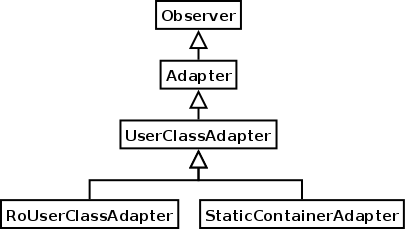
\includegraphics[width=7cm]{figs/png/adapuml}
\caption{\label{ADAPuml_f} Adapters class hierarchy}
\end{center}
\end{figure}



\subsubsection{Class \codename{Adapter}}
This is the base class for all adapters. All adapters derive from
class \codename{Observer}. Instantiation of an Adapter can be
optionally complex and customizable by using same optional
parameters. Available parameters are presented here, but examples
will show them applied in a practical manner. 

Important operations are:

\begin{description}
\item [Constructor] Class constructor gets several parameters, but
  only two are strictly required.
{
\codesize
\begin{verbatim}
def __init__(self, model, prop_name, 
             prop_read=None, prop_write=None, 
             value_error=None)
\end{verbatim}
}

\begin{description}
  \item [\codename{model}] is the Model instance containing the
    property to be observed.

  \item [\codename{prop\_name}] is the model's property name (as a
    string). It is possible to use a dotted notation to identify a
    property contained into a hierarchy of models. For example
    'a.b.c' identifies property 'c' into model 'b' inside model 'a',
    where model 'a' is an attribute of given top level model. Last
    name can be an observable or non-observable attribute, and
    previous names (if specified) must all refer to instances of
    class \codename{Model}. First name from the left must be the
    name of a model instance inside the given model.

  \item [\codename{prop\_read}] optional function that apply custom
    modifications to the value of the property before reading
    it. The function takes a value and must return a transformed
    value. Use to customize the way the property is read, and to
    apply useful transformations to the read value.

  \item [\codename{prop\_write}] Like \codename{prop\_read} optional
    function that apply custom modifications to the value of the
    property before writing it. The function takes a value and must
    return a transformed value whose type must be compatible with
    the type of the property. Use to customize the way the property
    is written, and to apply useful transformations to the value.

  \item [\codename{value\_error}] optional parameter that can be a
    function (or a method) to be called when a \codename{ValueError}
    exception occurs while trying to set a wrong value for the
    property inside the model. The function will receive: the
    adapter, the property name and the value coming from the widget
    that offended the model. Useful to catch and handle error
    conditions.

\end{description}

\item [Widget connection] Constructor connects properties, while
  widgets are connected through method \codename{connect\_widget}:

{
\codesize
\begin{verbatim}
def connect_widget(self, widget,
                   getter=None, setter=None, 
                   signal=None, arg=None, update=True)
\end{verbatim}
}

\begin{description}

\item [widget] is the widget that is needed to connect
\item[getter] optional function used to ``read'' the
  widget. The function receives a widget instance.
\item[setter] optional function used to ``write'' the
  widget. The function receives a widget instance and the value to
  be written.
\item[signal] Optional name of the signal that will be used to
  monitor the widget changes.
\item[arg] Optional argument that is passed to the signal
  handler. It will be used when connecting the signal.
\item[update] If False, the widget will be not initially updated
  with the initial value of the property. Used in very particular
  conditions.
\end{description}

\item[update\_model()] Forces the property to be updated from the
  value hold by the widget. This method should be called directly by
  the user in very unusual conditions.

\item[update\_widget()] Forces the widget to be updated from the
  property value. This method should be called directly by the user
  when the property is not observable, or in very unusual conditions.

\end{description}


At this step thorough people would be asking them self how
instantiation of adapters can work in its simplest option, i.e. by
specifying the minimal set of parameters, and exploiting all default
values for the others.

The framework searches information about widgets and possible
default values for any unspecified parameter into module
\file{adapters.default}.

Suppose for example that the specified widget is a
\codename{gtk.Entry}. Good candidates for unspecified
\codename{getter} and \codename{setter} would be
\codename{gtk.Entry.get\_text} and \codename{gtk.Entry.set\_text}
respectively. \codename{signal} will be \codename{"changed"} to
capture events that change the value of the widget.

Later a list of all currently supported widgets will be presented.


\subsubsection{Class \codename{UserClassAdapter}}

This class handles the communication between a widget and a class
instance (possibly observable) that is a property inside the
model. The value to be shown is taken and stored by using a getter
and a setter. getter and setter can be: names of user class methods,
bound or unbound methods of the user class, or a function that will
receive the user class instance and possible arguments whose number
depends on whether it is a getter or a setter.

Class \codename{UserClassAdapter} derives directly from class
\codename{Adapter} and redefines the constructor as follow.

{
\codesize
\begin{verbatim}
  def __init__(self, model, prop_name,
               getter, setter, 
               prop_read=None, prop_write=None,                   
               value_error=None):
\end{verbatim}
}

Where \codename{getter} and \codename{setter} are two new required
parameters, and all the other are unchanged.

\begin{description}
\item [\codename{getter}] can be a string holding the name of the
  user class method, a bound or unbound method of the user class, or
  a function that will receive the user class instance. The function
  or method is required to return the value to be read into the user
  class.

\item [\codename{setter}] can be a string holding the name of the
  user class method, a bound or unbound method of the user class, or
  a function that will receive the user class instance and a value
  for setting. 
\end{description}



\subsubsection{Class \codename{StaticContainerAdapter}}
This class can be used to bound a set of widgets to a property that
is a container, like a tuple, a list or a map, or in general a class
that implements \codename{\_\_getitem\_\_} and
\codename{\_\_setitem\_\_} methods.

From the other hand, the set of widgets can be a list provided by
the user, or a container widget like a Box, a Notebook, etc.
Widgets will be linked by their position when the property is
list-like, or by their names or instances when the property is
map-like.

This class supports only properties that are static containers,
i.e. those containers that do not change their length
dynamically. If the container grows up in length, no change will
occur in the view-side.

This class derives from class \codename{UserClassAdapter}.

\begin{description}

\item [Widget connection] Different than Adapter's method,
  \codename{connect\_widget} accepts sets.

{ 
\codesize
\begin{verbatim}
def connect_widget(self, widget,
                   getters=None, setters=None, 
                   signals=None, arg=None)
\end{verbatim}
}

\begin{description}

\item [widget] is either a container widget, or a list of widgets. 
\item[getters] optional function or list or a map of functions used
  to ``read'' the widget(s). Each function receives a widget
  instance.
\item[setters] optional function or list or a map of functions used
  to ``write'' the widget(s). Each function receives a widget
  instance and value for setting.

\item[signal] can be None, a signal name, or a list or a map of
  signal names.

\item[arg] Optional argument that is passed to each signal
  handler. It will be used when connecting the signal(s). 
\end{description}

When maps are used, keys can be widgets or widget names. The length
of the possible lists or maps must be lesser or equal to the number
of widgets that will be connected.

\item[update\_model(idx=None)] Updates the value of property at
  given index. If \codename{idx} is \codename{None}, all controlled
  indices will be updated. This method should be called directly by
  the user in very unusual conditions.

\item[update\_widget(idx=None)] Forces the widget at given index to
  be updated from the property value. If index is not given, all
  controlled widgets will be updated. This method should be called
  directly by the user when the property is not observable, or in
  very unusual conditions.
\end{description}

Since things got a bit convoluted here, some examples can help to
understand how this kind of adapter can be used. 


Suppose you have a glade file containing a button and a
\codename{HBox} called \codename{"hbox"} containing a text entry, a
label and a \codename{SpinButton}.

\begin{figure}[here]
\begin{center}
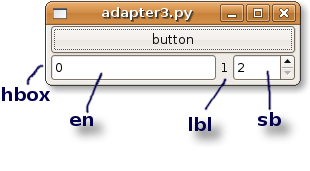
\includegraphics[width=4cm]{figs/png/adap2}
\caption{\label{ADAP2_f} \codename{StaticContainerAdapter} at work}
\end{center}
\end{figure}

The view is simply:

{ \codesize
  \begin{verbatim}
class MyView (View):
    def __init__(self, ctrl):
        View.__init__(self, ctrl, "adapters.glade", "window")
        return
    pass # end of class
  \end{verbatim}
}

The model contains a tuple of three integers that we want to connect
to the widgets into the \codename{HBox}. When the button is clicked,
one of the three integers is randomly incremented.

{ \codesize
  \begin{verbatim}
class MyModel (Model):
    __properties__ = {
       'box' : [0,1,2]
       }
    pass # end of class
  \end{verbatim}
}

The controller handles the button click signal:
{ \codesize
  \begin{verbatim}
import random
class MyCtrl (Controller):
    def on_button_clicked(self, button):
        self.model.box[random.randint(0,2)] += 1
        return
    pass # end of class
  \end{verbatim}
}

If typically construction of adapters occurs into method
\codename{register\_adapters} for the sake of simplicity in this
example instantiation of the adapter is located in the main
launching code:

{ \codesize
\begin{verbatim}
m = MyModel()
v = MyView()
c = MyCtrl(m, v)

a = StaticContainerAdapter(m, "box")
a.connect_widget(v["hbox"])

gtk.main()
\end{verbatim}
}

Adaption of widgets occur by their position into the
\codename{"hbox"} container. 

Second example makes use of an explicit list of widgets, and
exploits also parameter \codename{setters} to customize the way the
label \codename{"lbl"} shows its value.

{ \codesize
\begin{verbatim}
m = MyModel()
v = MyView()
c = MyCtrl(m, v)

a1 = StaticContainerAdapter(m, "box")
a1.connect_widget(map(lambda x: v[x], "en lbl sb".split()), 
                  setters = {'lbl': lambda w, v: 
                     w.set_markup("<big>Val: <b>%d</b></big>" % v)})

gtk.main()
\end{verbatim}
}

\begin{figure}[here]
\begin{center}
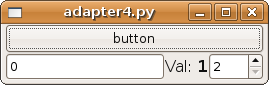
\includegraphics[width=4cm]{figs/png/adap3}
\caption{\label{ADAP3_f} Customized setter for the label}
\end{center}
\end{figure}


Finally, instead of being a tuple, the observable property can be
also a map, whose keys are widget names.

{ \codesize
\begin{verbatim}
class MyModel (Model):
    __properties__ = {
        'box' : { 'en'  : 0,
                  'lbl' : 1,
                  'sb'  : 2 }
        }
    pass # end of class
\end{verbatim}
}

in this case bounding between widgets and values into the property
in the model is carried out by looking at names, and not position.


\subsection{Support for adapter instantiation}
As already seen, since version 1.2 class \codename{Controller}
offers two new methods to support instantiation of adapters. 

\begin{description} 
\item [register\_adapters()] This method is called by the framework
  when it is the best time to create all adapters. All that users
  are required to do is to override this method into their
  controllers derived from \codename{Controller}.

\item [adapt(...)] This method can be used within
  \codename{register\_adapters} to adapt properties and
  widgets. Arguments can be one of the following:

  \begin{enumerate}
  \item Property name as a string. A corresponding widget is
    searched among view's widgets and if only one match is found, a
    default adapter is created. The type of the created adapter
    depends both on the property and the widget type. Widget name
    matching is performed by searching the property name into widget
    names, case insensitive.

  \item Property name and widget name. Like previous but widget name
    is explicitly declared.

  \item An instance of an Adapter. The adapter must be already
    connected to a widget.
  \end{enumerate}

  The first two flavors of method \codename{adapt} allows for an
  easy construction of a default adapter, but only the third allows
  for a full control.

\end{description}


\subsection{Supported widgets}
\label{SUPW}

Here follows the list of those widgets that are currently supported
by the framework out of the box. In method
\codename{Controller.adapt} when adapting a widget, it is searched
into this list a matching and one or more adapters are created.

If no matching is found, a fallback tentative is to connect to
widget signal \codename{"changed"} if there exists. If this fails,
an assertion is raised.

If a widget is not listed here, it does not mean that it is not
supported. Instead, it will be enough to specify all required
parameters when instantiating adapters.

\begin{center}
\begin{tabular}{|l|l|l|}
\hline
Widget type & Property type & Notes\\[0.5ex]
\hline
\codename{gtk.Arrow} & \codename{gtk.ArrowType} & Current direction\\
\codename{gtk.Calendar} & \codename{datetime} or \codename{date} & Selected day\\
\codename{gtk.CheckMenuItem} &  \codename{types.BooleanType} & Current toggle state\\
\codename{gtk.ColorButton} & \codename{gtk.gdk.Color}  & Selected colour \\
\codename{gtk.ColorSelection} & \codename{gtk.gdk.Color} & Selected colour\\
\codename{gtk.Entry} & String & Current entry content \\
\codename{gtk.Expander} &  \codename{types.BooleanType} & True if expanded\\
\codename{gtk.Label} & String or number & Label content \\
\codename{gtk.ToggleButton} &  \codename{types.BooleanType} & Current toggle state \\
\hline
\end{tabular} 
\end{center}



% ----------------------------------------------------------------------

\newpage
% ----------------------------------------------------------------------
\section{progen: A Project Generator}

Since version 1.2 a little application called \kw{gtkmvc-progen}
is provided. Goal of \kw{gtkmvc-progen} is to generate the skeleton
of a project that can be used when starting up a new application
based on gtkmvc.

\kw{gtkmvc-progen} creates a directory containing the skeleton of a
new project, called the top-level directory.

The newly created project is constituted by:
\begin{enumerate}
\item A source directory containing all project source code
\item An empty application-level Model
\item A simple application-level Controller
\item The application main View containing the application main window. 
\item A resources directory, containing for example the project
  glade files, but also possibly images, styles, and other resources
  loaded at runtime.
\item A launching script, localized in the top-level directory
\end{enumerate}


\kw{gtkmvc-progen} can be executed as a batch program to be
controlled from the command line, or as a simple GUI
application. \kw{gtkmvc-progen} is of course based on \pygtkmvc. All
the work is performed by the model, and a view and a controller are
loaded when a GUI is required. Depending on the hosting platform,
\kw{gtkmvc-progen} is launched by default either in batch or in GUI
mode. Unix users are more familiar with command-line programs, and
will find \kw{gtkmvc-progen} to be executed in that modality by
default. Windows users will find the GUI presented by default
instead.

The way \kw{gtkmvc-progen} can be customized is by setting some
properties inside the model, either by using the command line, or by
using the GUI that does not export the full set of properties,
though.

Here is the list of properties with a short description:

\begin{center}
\begin{tabular}{|l|l|l|l|}
\hline
Property name& Property type & Description & Default value\\[0.5ex]
\hline
name & string & name of the project & \textbf{REQUIRED} \\
author & string & Developer's name & \textbf{REQUIRED} \\
email & string & Developer's email address & \\
copyright & string & Copyright string & A sensible string\\
destdir & string & name of destination directory & "." \\
complex & bool & Generates hierarchical MVC support & True \\
dist\_gtkmvc & bool & If True, gtkmvc is embedded & True \\
glade & bool & if glade files are going to be used or not & True \\
\hline
glade\_fn & string & filename of generated glade file & application.glade \\
src\_header & string,None & Template for source header files. & None \\
other\_comment & string & Additional comment pushed after headers &  \\ 
src\_name & string & Name of the source directory & "src" \\
res\_name & string & Name of the resources directory & "resources" \\
top\_widget & string & Name of the View's top-level widget & "window\_appl" \\
\hline
\end{tabular} 
\end{center}

Bottom part of the table contains less important properties. Python
module \file{gtkmv.progen.templates} contains default templates that
are used for headers, license, etc. 

Boolean option \kw{gui} can be used to select batch or gui
mode. Option \kw{help} can be used to print out an helping message.

\bigskip

\kw{gtkmvc-progen} can be executed either locally from the script
directory, or can be executed as any other program if \pygtkmvc has
been properly installed on the hosting system.

From the local script directory:
\begin{verbatim}
$> python gtkmvc-progen param=val ...
\end{verbatim}

If \pygtkmvc was installed:
\begin{verbatim}
$> gtkmvc-progen param=val ...
\end{verbatim}

Boolean properties can be specified in the form ``param'' or in the
form ``param=[yes|no]''. Specifying boolean ``param'' or
``param=yes'' is semantically equivalent.

For example:
\begin{verbatim}
$> gtkmvc-progen name=hello author="Roberto Cavada" gui glade=no
\end{verbatim}

The result is the creation of the top-level directory whose name is
the project name. Inside a top-level script can be used to launch
the application. 

% ----------------------------------------------------------------------

\end{document}
